% This is samplepaper.tex, a sample chapter demonstrating the
% LLNCS macro package for Springer Computer Science proceedings;
% Version 2.20 of 2017/10/04
%
\documentclass[runningheads]{llncs}
%
\usepackage{graphicx}
\usepackage{subfig}
% Used for displaying a sample figure. If possible, figure files should
% be included in EPS format.
%
% If you use the hyperref package, please uncomment the following line
% to display URLs in blue roman font according to Springer's eBook style:
% \renewcommand\UrlFont{\color{blue}\rmfamily}
%
% Git commands:
%
% git commit -a
% git push



\begin{document}
%
\title{Understanding Input Data Requirements and Quantifying Uncertainty for Successfully Modelling `Smart' Cities 
\thanks{This work was supported by a European Research Council (ERC) Starting Grant [number 757455], a UK Economic and Social Research Council (ESRC) Future Research Leaders grant [number ES/L009900/1], an ESRC-Alan Turing Fellowship [ES/R007918/1] and through an internship funded by the UK Leeds Institute for Data Analytics (LIDA).}}

%
\titlerunning{Data Requirements for Modelling Cities}
% If the paper title is too long for the running head, you can set
% an abbreviated paper title here
%

\author{Nick Malleson\inst{1,3}\orcidID{0000-0002-6977-0615} \and
Jonathan A. Ward\inst{2}\orcidID{0000-0003-3726-9217} \and
Alison Heppenstall\inst{1,3}\orcidID{0000-0002-0663-3437} \and
Michael Adcock\inst{3} \and
Daniel Tang\inst{4}  \and
Jonathan Coello\inst{4} \and
Tomas Crols\inst{1,3}\orcidID{0000-0002-9379-7770}
}
%

\authorrunning{Malleson et al.}
% First names are abbreviated in the running head.
% If there are more than two authors, 'et al.' is used.
%
\institute{
School of Geography, University of Leeds, LS2 9JT, UK \\
\url{http://geog.leeds.ac.uk/} \\
\email{n.s.malleson@leeds.ac.uk} 
 \and
School of Mathematics, University of Leeds, LS2 9JT, UK \\
\url{http://maths.leeds.ac.uk} 
\and
Leeds Institute for Data Analytics (LIDA), University of Leeds, LS2 9JT, UK \\
\url{http://lida.leeds.ac.uk} \and
Improbable, 30 Farringdon Road, London, EC1M 3HE, UK \\
\url{http://www.improbable.io}
}
%
\maketitle              % typeset the header of the contribution
%
\begin{abstract}

Agent-based modelling (ABM) is ideally suited to modelling the behaviour and evolution of social systems. However, there is inevitably a high degree of uncertainty in projections of social systems -- input data are noisy and sparse, and human behaviour is itself extremely uncertain -- one of the key challenges facing the discipline is the quantification of uncertainty within the outputs of agent-based models. Without an adequate understanding of model uncertainty, or a means to better constrain models to reality, simulations will naturally diverge from the target system.  This limits the value of their predictions.
This paper presents ongoing work towards methods that will (i) allow real-time data to be assimilated into models to reduce the uncertainty of their predictions and to (ii) quantify the \textit{amount} of data (including overall volume as well as spatio-temporal granularity and regularity) that are required for successful assimilation (i.e. to model the system within an acceptable level of uncertainty).
Specifically, this project emulates a simple system of pedestrians who all move towards an exit. The paper reports on initial experiments to constrain the range of possible model outcomes using Bayesian inference techniques as implemented in a new probabilistic programming library. 
Ultimately the project aims to provide valuable information about the number and type of sensors that might be required to model movements of humans around real urban systems.

\keywords{Agent-based modelling \and Uncertainty \and Data assimilation \and Bayesian inference}
\end{abstract}
%
%
%
 

\section{Introduction and Background}

Individual-level modelling approaches, such as agent-based modelling (ABM), are ideally suited to modelling the behaviour and evolution of social systems. This is especially true in the context of modern `smart' cities, where large volumes of data, supported by innovative `big' data analytics, can be leveraged to better understand and capture the characteristics of the underlying systems. However, there is inevitably a high degree of uncertainty in projections of social systems -- input data are noisy and sparse, and human behaviour is itself extremely uncertain -- one of the key challenges facing the discipline is the quantification of uncertainty within the outputs of these models.

This work focusses on the simulation of \textit{urban flows}, i.e. the movement of people around urban areas over relatively short time scales (minutes and hours). It presents ongoing work towards methods that will (i) allow real-time data to be assimilated into models to reduce the uncertainty of their predictions and (ii) to quantify the \textit{amount} of data (including overall volume as well as spatio-temporal granularity and regularity) that are required for successful assimilation. In other words, given some human system and a simulation of that system (we study the movement of pedestrians in this case), how much data are required from the real system in order to prevent the model uncertainties from causing the simulation to rapidly diverge from reality? With too little data it will be impossible to reliably constrain the model to reality, but how much is too little? Is one well-placed footfall counter sufficient to capture the dynamics of the system, or in reality would it be necessary to track the actual movements of a large proportion of the individual people? The hypothetical model used here is a simple system of pedestrians, each of whom move from an entrance towards one of two exits. This is analogous to a train arriving at a train station and passengers moving across the concourse to leave. The model environment is illustrated in Figure~\ref{fig:pedestrian_model_environment}. 

%It will  experiment with methods that are common in other fields, such as 4D-Var, and (Ensemble) Kalman Filtering, and could be leveraged for ABM to assimilate streams of new data into running models in order to reduce uncertainty. For example, Figure~\ref{fig:ensemble_uncertainty} illustrates one way that models of weather systems use ensembles to quantify the uncertainty associated with forecasts. 
%
%\begin{figure}
%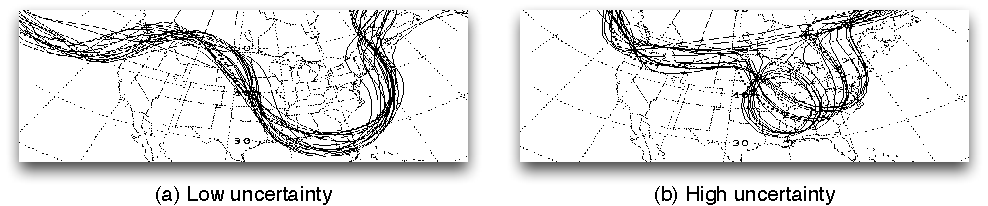
\includegraphics[width=\textwidth]{figures/ensemble_uncertainty}
%\caption{A `spaghetti plot' illustrating pressure contours as forecast from numerous models in an ensemble. Adapted from~\cite{kalnay_atmospheric_2003}. In (a), the results across different models are similar and hence the forecast has relatively low uncertainty. In (b), however, the results vary substantially in some areas so the forecast is less certain} \label{fig:ensemble_uncertainty}
%\end{figure}

% There is very limited prior work in which data is assimilated iteratively into typical agent-based models. 
Very limited prior work has been conducted in this area. Some authors have attempted to conduct data assimilation, but use agent-based models that are simple in the extreme~\cite{malleson_forecasting_2017,ward_dynamic_2016}. Here, a more advanced model will be used in order to test how well the various methods handle complex features such as emergence and feedback. Others have developed more complex agent-based models~\cite{flotterod_bayesian_2011} but those must remain mathematically coupled to an aggregate proxy model which limits the flexibility of the underlying agent-based model. The most similar work is that of \cite{wang_data_2015}, who attempt to assimilate data into a model of peoples' movement in buildings. They do this by running an ensemble of models and re-starting each one using new input conditions that are created each time new data become available. The main difference between the approach in \cite{wang_data_2015} and this paper is that here the aim is to eventually develop methods that are able to assimilate new data that automatically \textit{alter the state} of the simulation while it is running. This is more analogous with data assimilation techniques in other fields \cite{kalnay_atmospheric_2003}.

%There are a range of established methods, commonly used in the physical sciences, that have been developed to reduce the uncertainty in forecasts by assimilating up-to-date information about the physical system that they are attempting to represent. These include Successive Corrections Method, Optimal Interpolation, 3D-Var, 4D-Var, and (Ensemble) Kalman Filtering (see \citep{kalnay_atmospheric_2003} for a good review). However, many of these methods have been applied in the context of models are typically based on systems of aggregate differential equations, with functions linearised mathematically, so make assumptions about the linearity of their underlying models that might not apply to agent-based models. 



\begin{figure}
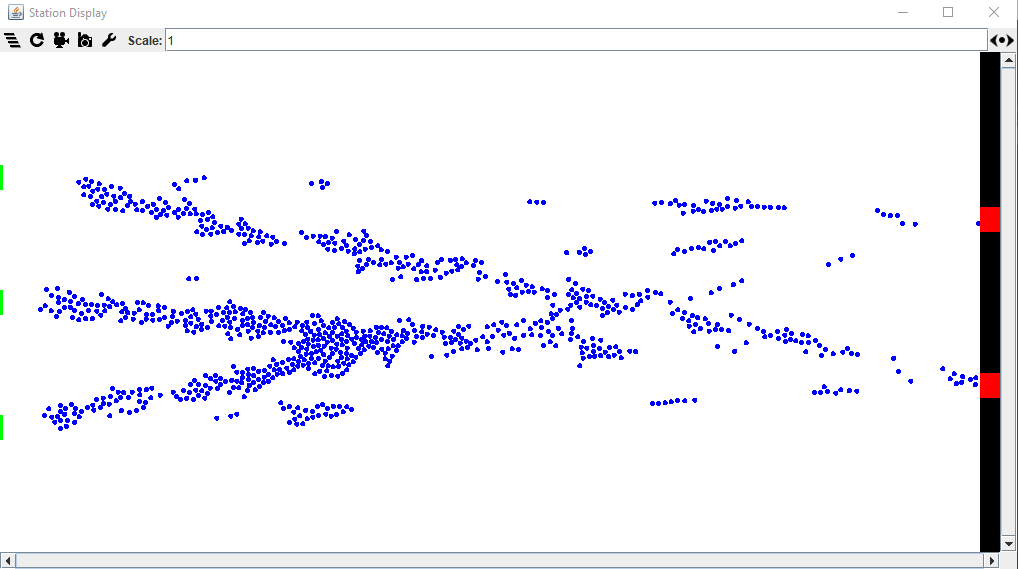
\includegraphics[width=\textwidth]{figures/pedestrian_model_environment}
\caption{A snapshot of the simple, hypothetical model that is used here. Agents arrive from the green entrances on the left and move towards the red exits on the right.} \label{fig:pedestrian_model_environment}
\end{figure}

\section{Methods}

\subsection{Overall Approach}

This paper presents a work in progress, whose overall proposed approach is to:

\begin{enumerate}
\item Develop a  agent-based simulation of pedestrian movements from an entrance to an exit using a simple social forces framework (similar to \cite{helbing_social_1995}) to control the behaviour of the agents (see Figure~\ref{fig:pedestrian_model_environment});
\item Run the simulation to generate hypothetical `truth' data, our equivalent reality created with synthetic data. We assume this equivalent reality represents the real underlying system.  We sample from this in a manner analogous to that of using sensors of peoples' movements to sample from the real world;
\item \label{objectives:current} Re-run the simulation with a different random seed and use samples of varying resolution from the `truth' data to reduce the uncertainty of the new simulation;
\item \label{objectives:da} Quantify the volume (total number of samples), granularity (amount of aggregation) and regularity (the number of samples per time period) that are required to successfully model the hypothetical `real' data.
\end{enumerate}

This paper presents the preliminary results up to stage \ref{objectives:current}, with the ultimate aim of quantifying the amount of data required to successfully constrain the simulation being immediate future work. 


\subsection{Preliminary Results: Constraining Model Uncertainty}

Our initial experiments use a prototype probabilistic programming library to perform parameter estimation using Bayesian inference (see \cite{ghahramani_probabilistic_2015} for a useful discussion about probabilistic programming and Bayesian inference). This work is a precursor to performing data assimilation (i.e. step \ref{objectives:da}). The probabilistic programming approach treats the pedestrian simulation as a black box, whose only \emph{input} is a list of random numbers that are used in the simulation whenever a probabilistic decision is made and whose \emph{output} is the number of agents in the system at each time step. All internal simulation parameters are fixed. The simulation output is deterministic given the same input, but different inputs result in different outputs, and so stochastic simulations can be performed by choosing the input at random. Figure~\ref{fig:procedure_diagram} illustrates the method. 

We create truth data, i.e. agent counts over time, from a single model run using a model input (a list of random decimal numbers) sampled from a Gaussian distribution. Then, using a noisy observation of the truth data, we use the probabilistic programming library to create a Bayesian network from which we can compute the posterior distribution of the input given the noisy observation. We then sample from this distribution using Metropolis-Hastings, resulting in an ensemble of model realisations in which the uncertainty of the input, and hence the output, is constrained.

%% Parameter estimation was accomplished by configuring the model such that all parameters were fixed, with the only input being a list of random numbers that the model uses each time a probabilistic decision needs to be made. If the model uses all of these random numbers and requires another, it recycles from the beginning of the list. (Note that if only one random number to be passed to the model then every run would be identical as all probabilistic decisions would become stochastic). The output of the model is a list that specifies the number of agents in the simulation at each time step. This varies with each simulation because crowding can occur at random depending on the speed that different agents travel in the simulation and the exits that they are moving towards. In the future, different types of output that describe the hypothetical 'real' world in more or less detail will be experimented with to ascertain which have enough information to constrain the simulation adequately.

\begin{figure}%
\centering
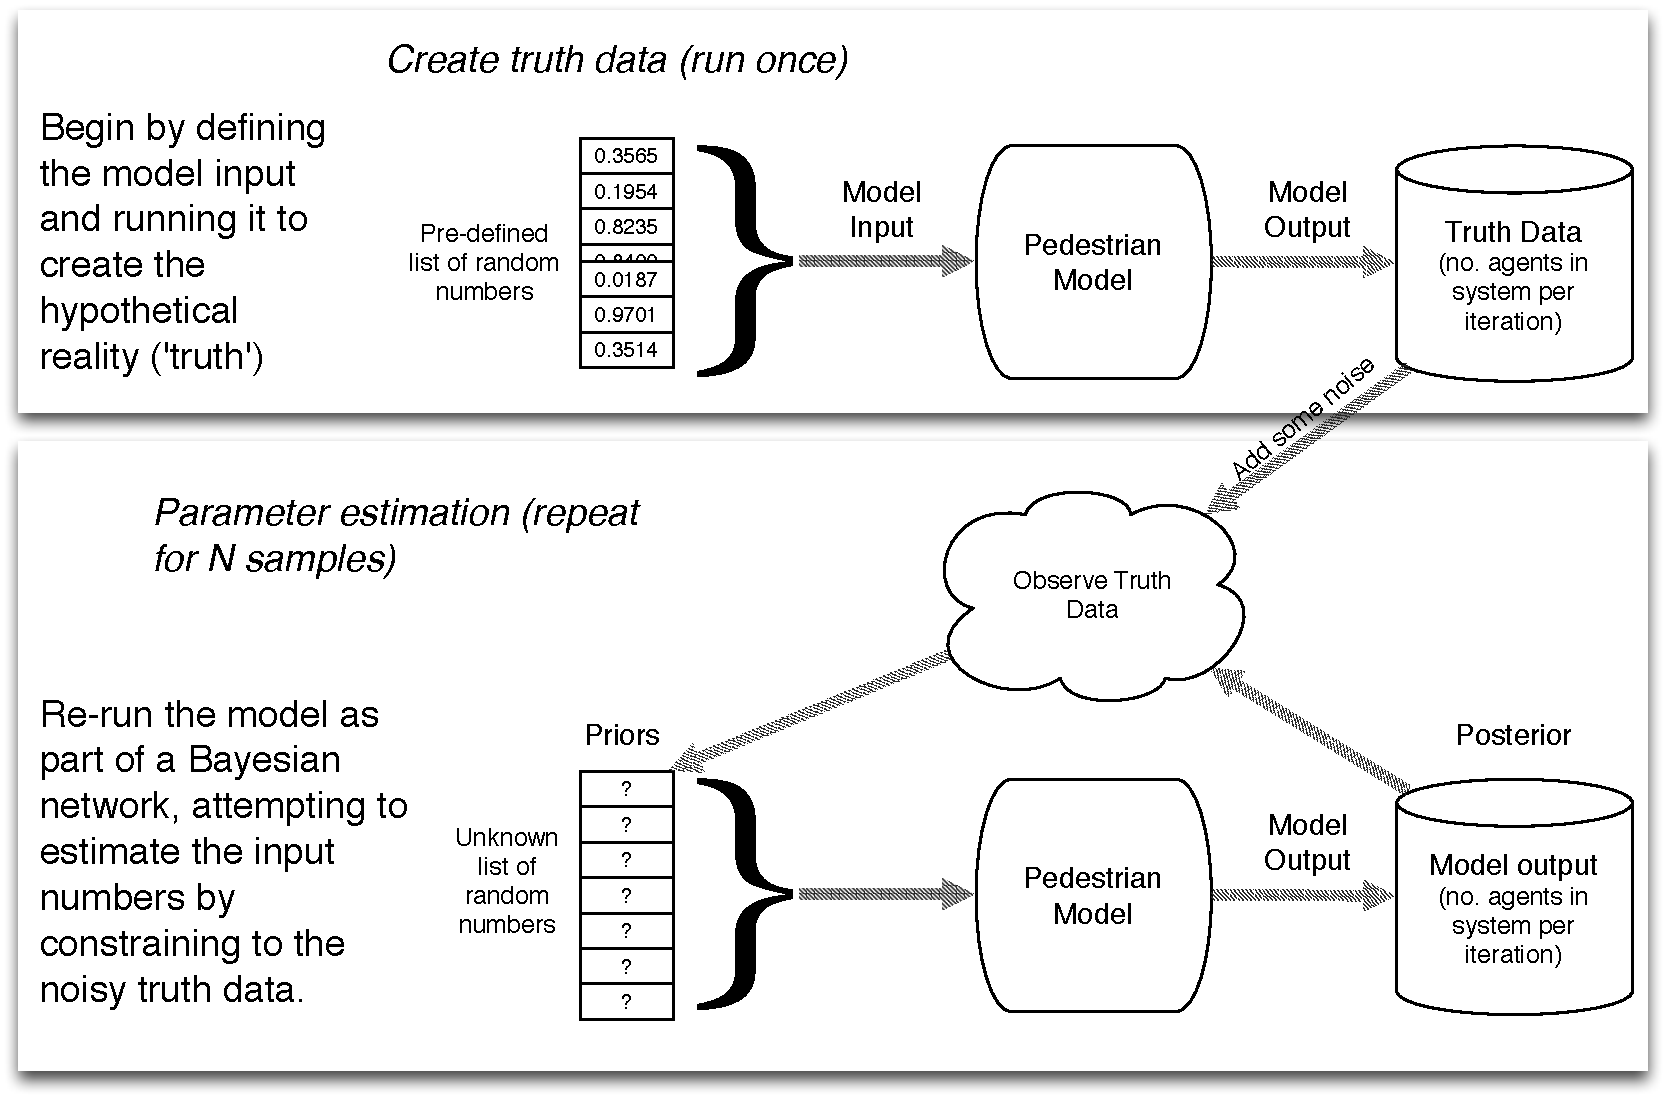
\includegraphics[width=\textwidth]{figures/procedure_diagram}
\caption{An illustration of the procedure to perform parameter estimation.} 
\label{fig:procedure_diagram}
\end{figure}




%% A list of $100$ random numbers (i.e. the model input) were created and these were passed to the model to create the `truth' data. Following this, the model was integrated into a Bayesian network and the posterior distribution (the simulated number of agents in the system at each time step) was sampled. Importantly, two sampling routines were executed: one that used the truth data to attempt to constrain the posterior distribution by accurately estimating the values of the original random numbers, and another that did not include this observation step.

Figure~\ref{fig:model_uncertainty} compares the results of the sampling with and without the incorporation of the truth data. It is clear that when the Bayesian network makes use of the observations from the `truth' model, the output of each model (i.e. sample of the posterior distribution) is much more similar to the truth data. In other words, the procedure is more accurately estimating the list of random numbers (the prior distribution) that were initially used as input to generate the `truth' data. Although this result is not of value in isolation, it is very useful as a proof-of-concept. It shows that Bayesian inference on an agent-based model that has reasonably complex characteristics (namely the emergence of crowding due to agent interactions) is able to perform parameter estimation. More rigorous data assimilation is a relatively small step.

%\begin{figure}
%\includegraphics[width=\textwidth]{figures/results}
%\caption{An illustration of model uncertainty, produced using \textit{keanu} alpha release. Illustrates the number of people in the simulation across 50 different model runs (samples).} \label{fig:model_uncertainty}
%\end{figure}


\begin{figure}%
\centering
\subfloat[constrained to observations]{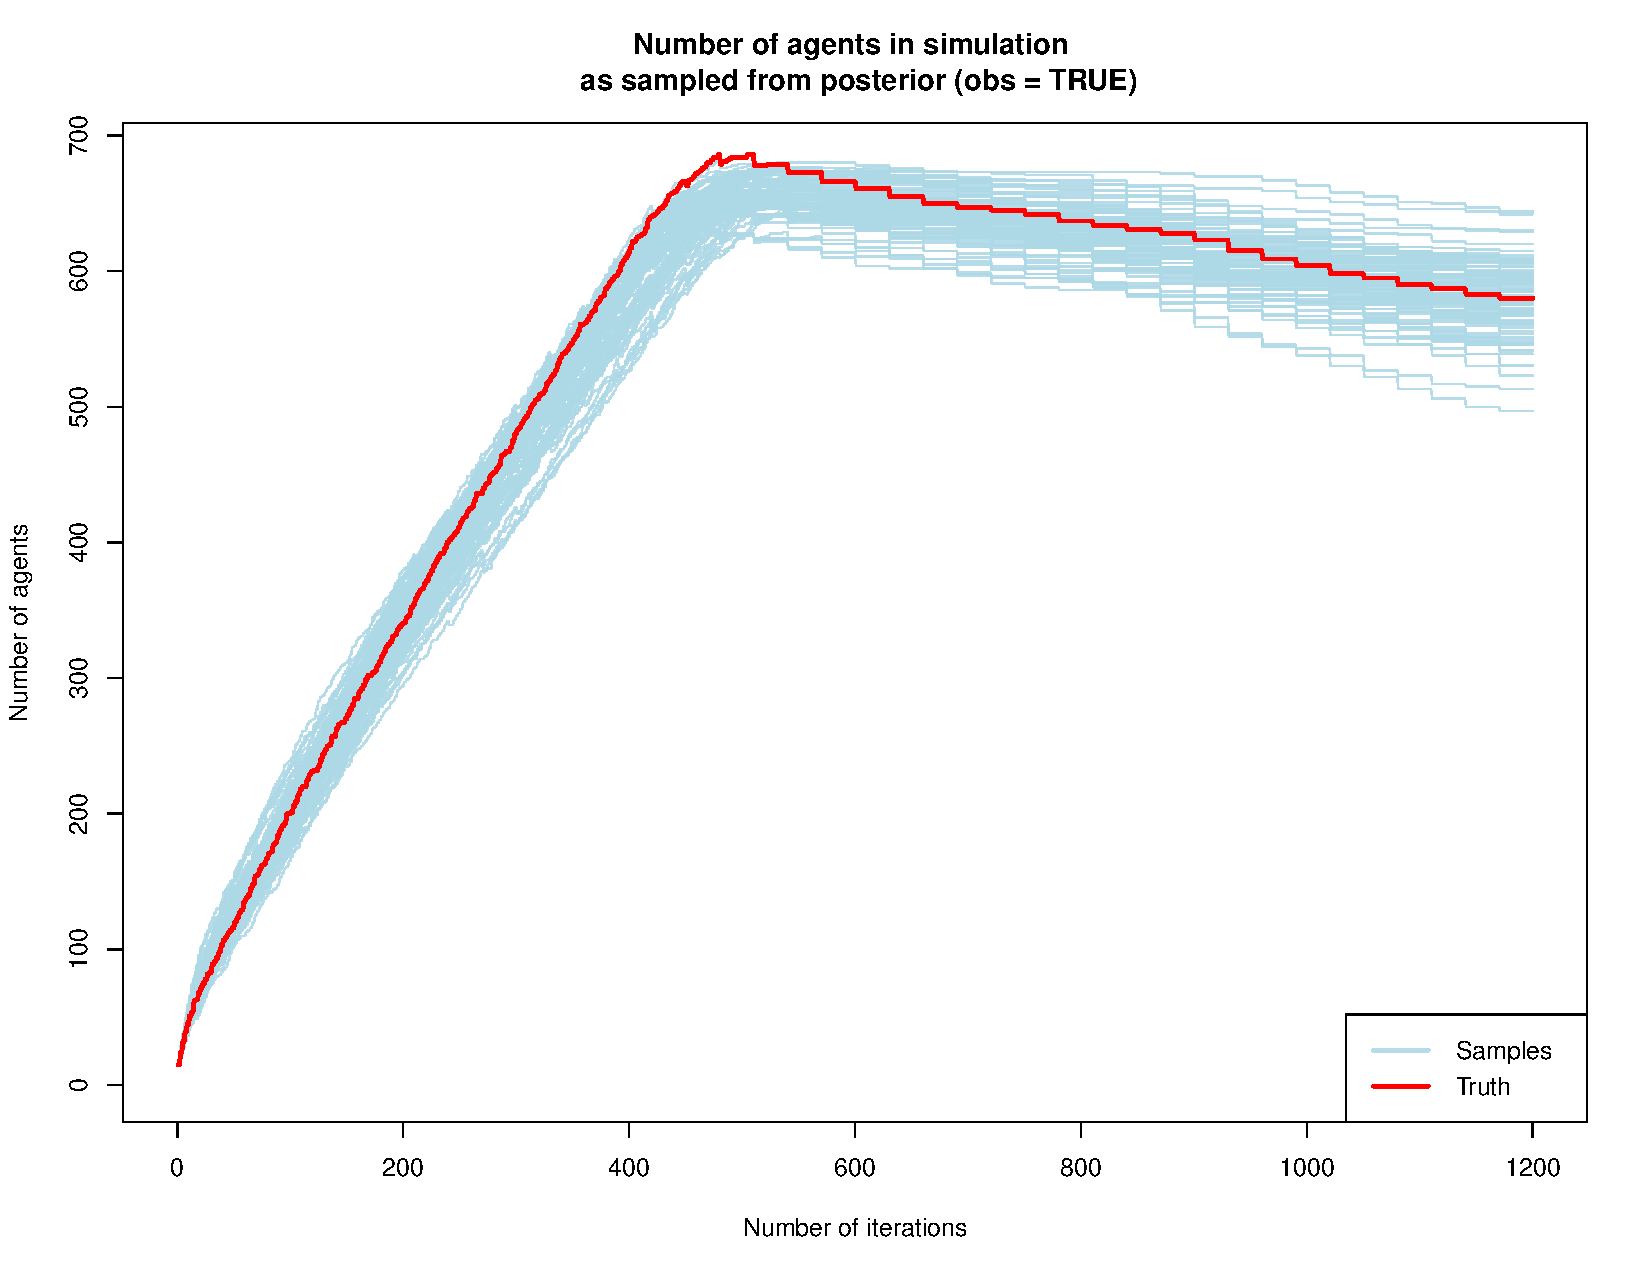
\includegraphics[width=0.49\textwidth]{figures/results-with_obs}\label{fig:results:with_obs}}
\subfloat[without observations]{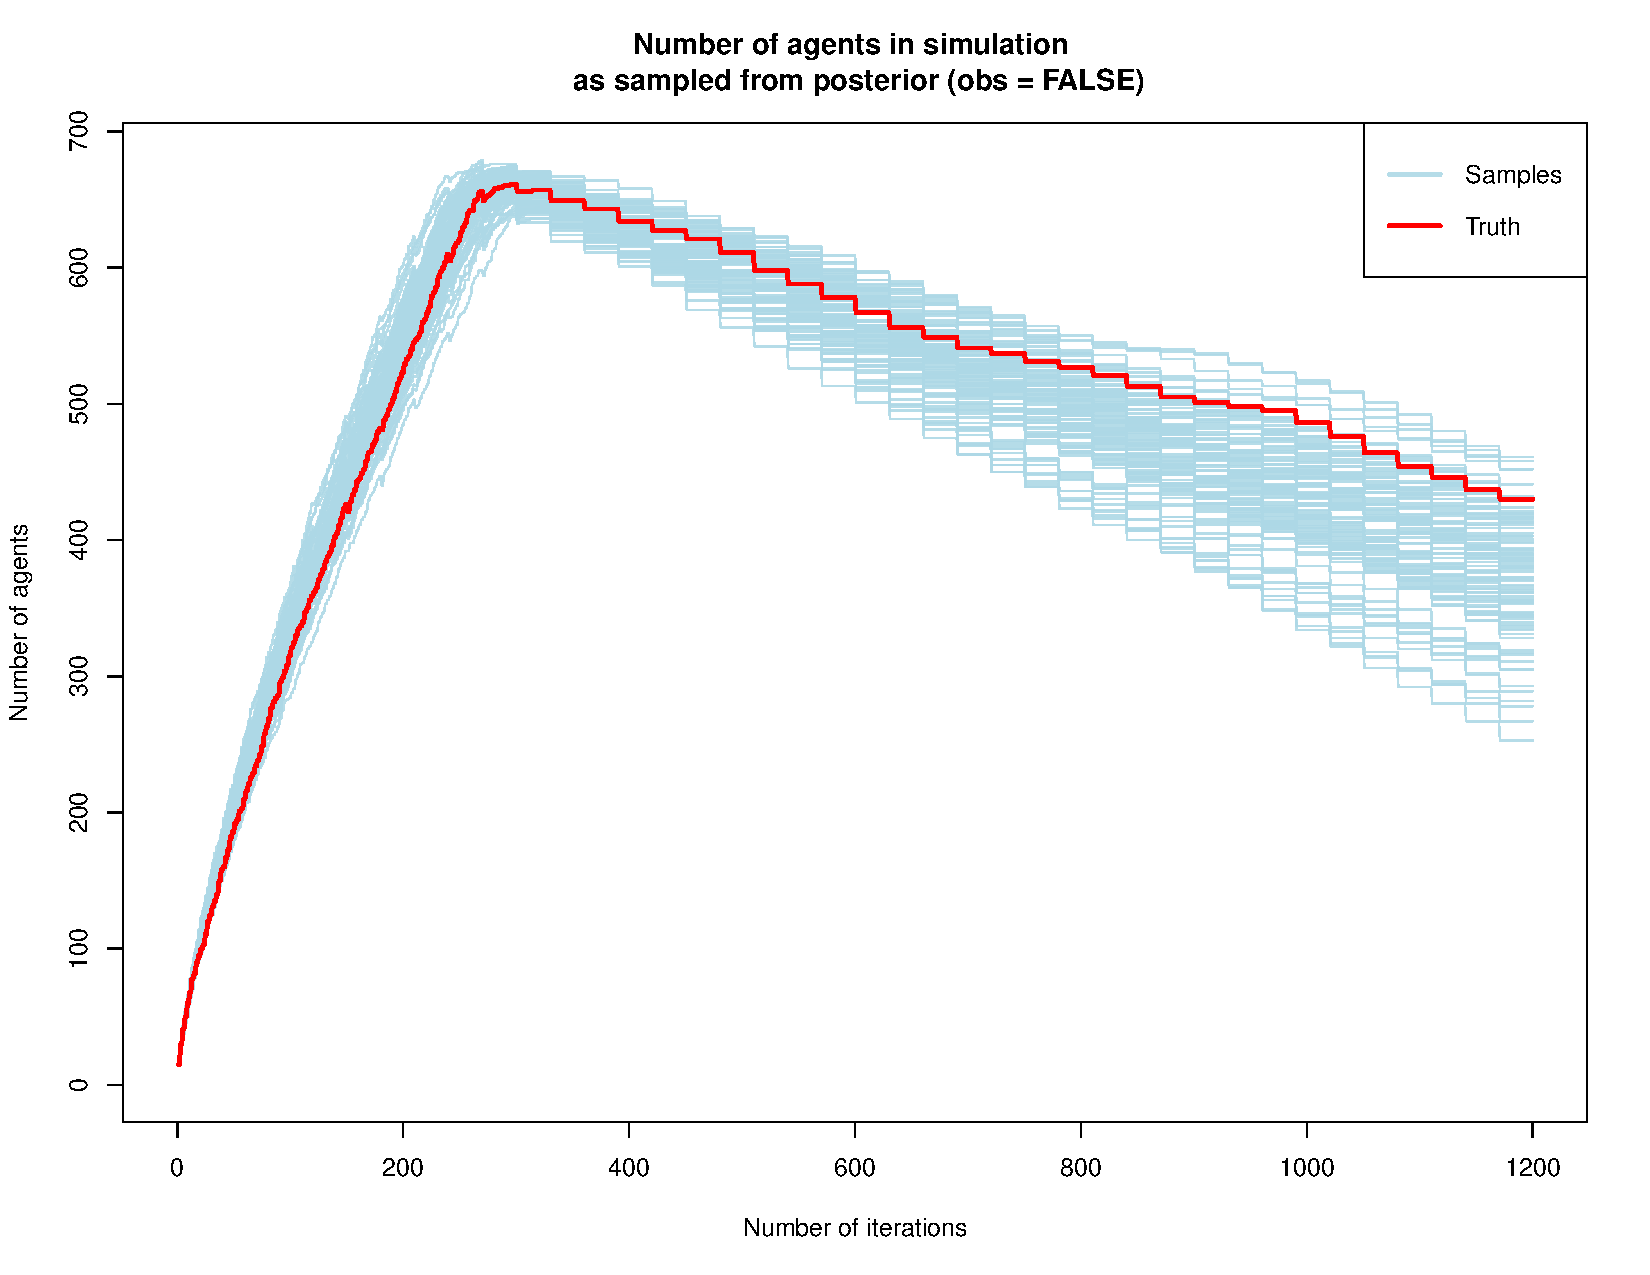
\includegraphics[width=0.49\textwidth]{figures/results-no_obs}\label{fig:results:no_obs}}
\caption{Results of sampling the posterior with observations (\ref{fig:results:with_obs}) and without (\ref{fig:results:no_obs}). When the `truth' data are used to constrain the posterior distribution, the sampling routine is much better able to estimate the input model state, so the outcomes of the samples are much closed to the `truth` data.} 
\label{fig:model_uncertainty}
\end{figure}


\section{Link to ABMUS Workshop Themes}

This paper addresses a core aspect of the ABMUS workshop theme; that of the \textit{trust} that we can have in model outputs. The conference recognises challenges in ``designing, developing and implementing \textbf{trusted} models that can be used by industry and governments to enhance decision-making''. By adapting existing methods that are aimed at reducing uncertainty in models through the incorporation of up-to-date data, this work advances the methodology towards more a rigorous representation of real urban systems that will be more acceptable for policy use.
%
%\section*{Appendix: Model Code and Parameters}
%
%\textit{I think I'll drop this section}
%
%For reproducibility, the model code, in full, is available at XXXX. The parameters used to generate the results here are provided in Table~\ref{tab:parameters}.
%
%\begin{table}[] \caption{Model parameters used to generate the results outlined here}
%\begin{center}
%\begin{tabular}{l p{0.5\textwidth} l}
%Parameter & Description & Value \\ \hline 
%numSamples & XX &  500 \\
%numTimeSteps & XX &  1200 \\
%numRandomDoubles & XX &  100 \\
%totalNumPeople & XX &  700 \\
%dropSamples & XX &  200 \\
%downSample & XX &  3 \\
%sigmaNoise & XX &  0.1 \\
%\end{tabular}
%\end{center} \label{tab:parameters} \end{table}%





%	
%
%  THE REST IS JUST EXAMPLES OF HOW TO USE THE LNCS STYLE
%
%
%\section{First Section}
%\subsection{A Subsection Sample}
%Please note that the first paragraph of a section or subsection is
%not indented. The first paragraph that follows a table, figure,
%equation etc. does not need an indent, either.
%
%Subsequent paragraphs, however, are indented.
%
%\subsubsection{Sample Heading (Third Level)} Only two levels of
%headings should be numbered. Lower level headings remain unnumbered;
%they are formatted as run-in headings.
%
%\paragraph{Sample Heading (Fourth Level)}
%The contribution should contain no more than four levels of
%headings. Table~\ref{tab1} gives a summary of all heading levels.
%
%\begin{table}
%\caption{Table captions should be placed above the
%tables.}\label{tab1}
%\begin{tabular}{|l|l|l|}
%\hline
%Heading level &  Example & Font size and style\\
%\hline
%Title (centered) &  {\Large\bfseries Lecture Notes} & 14 point, bold\\
%1st-level heading &  {\large\bfseries 1 Introduction} & 12 point, bold\\
%2nd-level heading & {\bfseries 2.1 Printing Area} & 10 point, bold\\
%3rd-level heading & {\bfseries Run-in Heading in Bold.} Text follows & 10 point, bold\\
%4th-level heading & {\itshape Lowest Level Heading.} Text follows & 10 point, italic\\
%\hline
%\end{tabular}
%\end{table}
%
%
%\noindent Displayed equations are centered and set on a separate
%line.
%\begin{equation}
%x + y = z
%\end{equation}
%Please try to avoid rasterized images for line-art diagrams and
%schemas. Whenever possible, use vector graphics instead (see
%Fig.~\ref{fig1}).
%
%\begin{figure}
%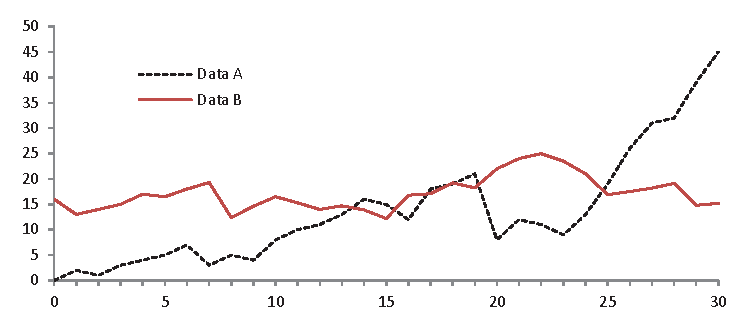
\includegraphics[width=\textwidth]{figures/fig1.eps}
%\caption{A figure caption is always placed below the illustration.
%Please note that short captions are centered, while long ones are
%justified by the macro package automatically.} \label{fig1}
%\end{figure}
%
%\begin{theorem}
%This is a sample theorem. The run-in heading is set in bold, while
%the following text appears in italics. Definitions, lemmas,
%propositions, and corollaries are styled the same way.
%\end{theorem}
%%
%% the environments 'definition', 'lemma', 'proposition', 'corollary',
%% 'remark', and 'example' are defined in the LLNCS documentclass as well.
%%
%\begin{proof}
%Proofs, examples, and remarks have the initial word in italics,
%while the following text appears in normal font.
%\end{proof}
%For citations of references, we prefer the use of square brackets
%and consecutive numbers. Citations using labels or the author/year
%convention are also acceptable. The following bibliography provides
%a sample reference list with entries for journal
%articles~\cite{ref_article1}, an LNCS chapter~\cite{ref_lncs1}, a
%book~\cite{ref_book1}, proceedings without editors~\cite{ref_proc1},
%and a homepage~\cite{ref_url1}. Multiple citations are grouped
%\cite{ref_article1,ref_lncs1,ref_book1},
%\cite{ref_article1,ref_book1,ref_proc1,ref_url1}.
%
% ---- Bibliography ----
%
% BibTeX users should specify bibliography style 'splncs04'.
% References will then be sorted and formatted in the correct style.
%

\bibliographystyle{splncs04}
\bibliography{2018-abmus-abm_uncertainty}

\end{document}
